% !TEX program = lualatex
% !TEX options = -synctex=1 -interaction=nonstopmode -file-line-error -shell-escape -output-directory=%OUTDIR% "%DOC%"

\documentclass[12pt, a4paper]{article}
\usepackage{amsfonts}
\usepackage{amssymb}
\usepackage{amsmath}
\usepackage[english]{babel}
\usepackage{caption}
\usepackage{float}
\usepackage[left=2cm, top=2cm, right=2cm, bottom=2cm]{geometry}
\usepackage{graphicx}
\usepackage{listings}
\usepackage[newfloat, outputdir=out_tex]{minted}
\usepackage{pgf}
\usepackage{pdfpages}

\graphicspath{{figures/}}

\setlength\parindent{0pt}

\newcounter{lstNoteCounter}
\SetupFloatingEnvironment{listing}{name=Source code}


\begin{document}
  \centerline{\Huge\scshape Computational physics}
  \vspace*{0.5cm}
  \hrule
  \vspace*{0.5cm}
  \centerline{Jona Ackerschott, Julian Mayr}
  \vspace*{1cm}
  \centerline{\Large\bfseries Problem set 6}
  \vspace*{0.5cm}

  \section*{Problem 1}
  Copying the given Mathematica code into our own notebook returns a plot of the numerical solution
  
  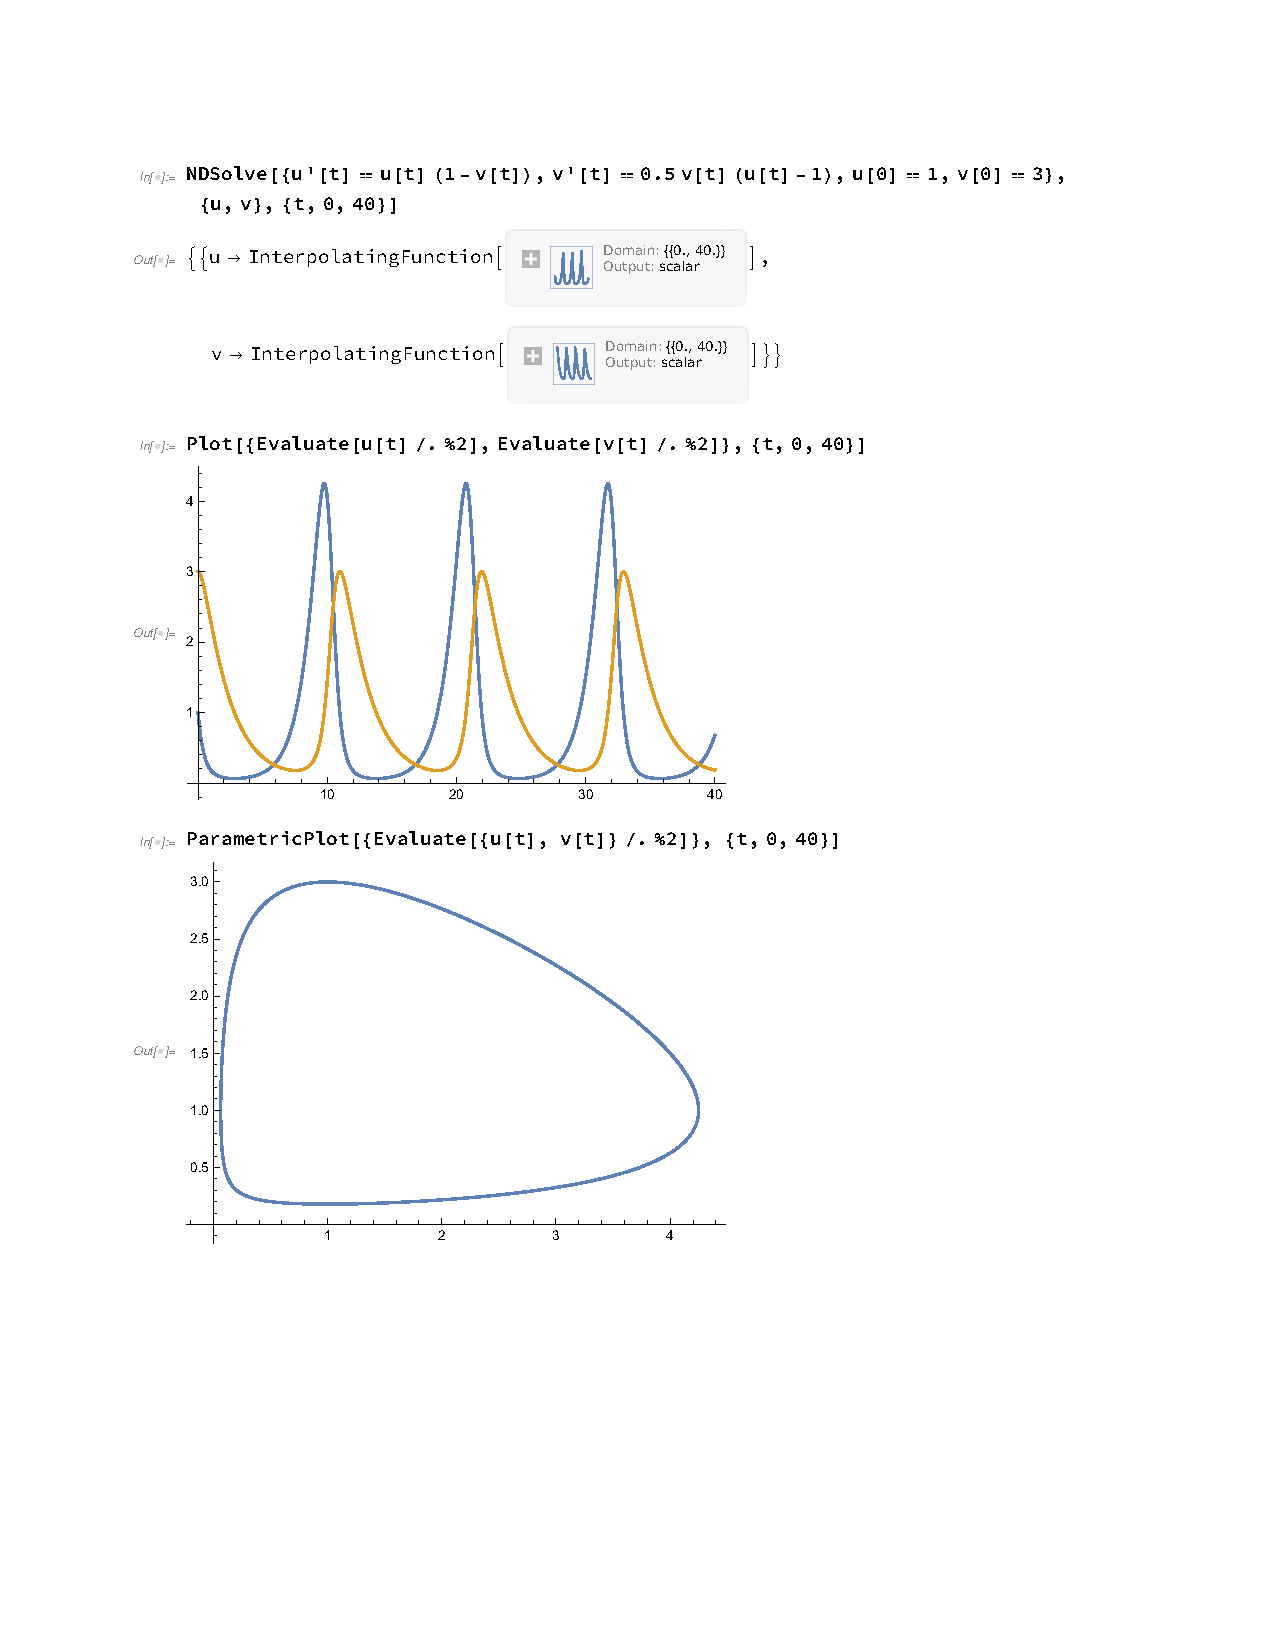
\includegraphics[scale=0.6,page=1]{nb1.pdf}
  
  The function $NDSolve$ creates an object which contains Mathematica's numerical interpretation of the ODE. This object can be evaluated using $Evaluate$, and then plotted using $Plot$, or $ParametricPlot$ for a parametric plot.
\\This can also be used to solve vector valued differential equations, like the 2-body-problem. This was done in the following notebook:

  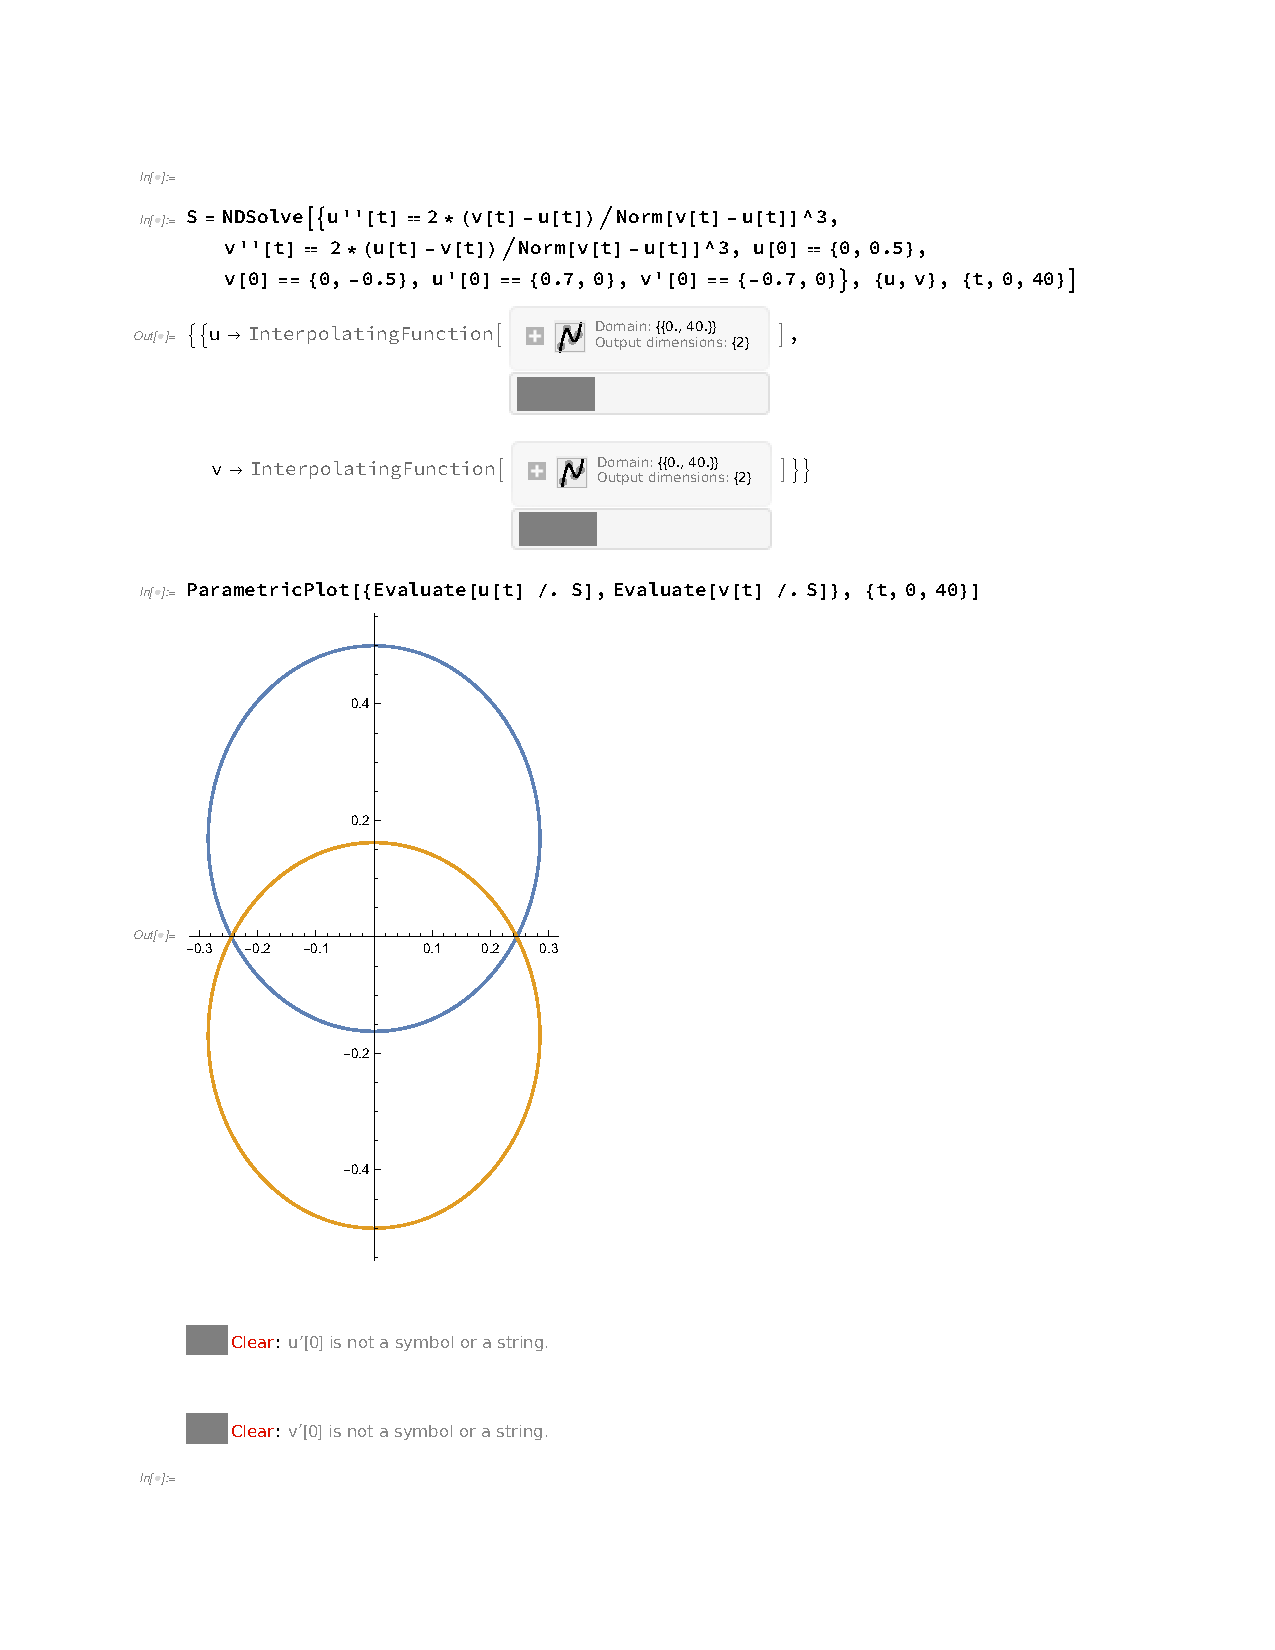
\includegraphics[scale=0.6, page=1, trim=0 200 0 0, clip]{2body.pdf}

  The typical 2-Body-Problem Movement can be seen clearly. There is also no euler-like error to be seen, because $NDSolve$ uses a pretty complex combination of ODE solving algorithms. For additional accuracy, $PrecisionGoal$ and $AccuracGoal$ variables can be given, though they are not necessary for this problem.
  \section*{Problem 2}
  Through examination of the population dynamics equation
  \begin{align}
    \frac{{\rm d} N}{{\rm d} t} = r N (1 - N / K) - \frac{B N^2}{A^2+N^2}
    \label{eq_population_dynamic_de}
  \end{align}
  one sees immediately, using the dimensions of N (dimension: count, here named C) and t (dimension: time, here named T) that $[r] = \frac{1}{C T}$, $[K] = C$, $[A] = C$ and $[B] = \frac{C}{T}$. So with the definitions $\kappa = \frac{K}{A}$, $\varrho = \frac{A}{B} r$, $\tau = \frac{B}{A} t$ and $n = \frac{N}{A}$ one obtains a dimensionless form of (\ref{eq_population_dynamic_de}).
  \begin{align}
    \frac{{\rm d} n}{{\rm d} \tau} = \varrho n \left(1 - \frac{n}{\kappa} \right)
      - \frac{n^2}{1 + n^2}
    \label{eq_population_dynamic_de_dimless}
  \end{align}
  From that stationary points can be found by imposing $\frac{{\rm d} n}{{\rm d} \tau} = 0$
  \begin{align}
    & \varrho n \left(1 - \frac{n}{\kappa} \right)
      - \frac{n^2}{1 + n^2} = 0 \nonumber \\
    \Leftrightarrow \ & \varrho n \left(1 - \frac{1}{\kappa} n + n^2
      - \frac{1}{\kappa} n^3 \right) - n^2 = 0 \nonumber \\
    \Leftrightarrow \ & n^3 - \kappa n^2
      + \left(1 + \frac{\kappa}{\varrho}\right) n - \kappa = 0
    \label{eq_polynom_stationary}
  \end{align}
  Now while setting $\kappa = 7.5$, one can compute the zeros or rather the stationary points from this equation, for a specific value for $\varrho$, by applying the Mathematica method \texttt{NRoots} on (\ref{eq_polynom_stationary}). For values of $\varrho$ from $-1$ to $1$ this leads to the plot shown in figure \ref{fig_stationary_points}.

  \begin{figure}[h]
    \centering
    \includegraphics[width=0.75\textwidth]{fig2_1.pdf}
    \caption{Stationary points of (\ref{eq_population_dynamic_de_dimless}) in dependence of the parameter $\varrho$. If the plot is multivalued there exists more than one solution to (\ref{eq_polynom_stationary})}
    \label{fig_stationary_points}
  \end{figure}

  This graph also shows the points at which the number of solution changes from $1$ to $3$ (or rather from $1$ to $2$ to $3$) or reversed.

  The stability of the stationary points can be determined by the sign of the derivative of (\ref{eq_polynom_stationary}) with respect to $n$ at the specific root. The derivative at the respective points can be determined in Mathematica as well and a plot of these derivative for each value of $\varrho$ from -1 to 1 is shown below in figure \ref{fig_stationary_points_stability}.

  \begin{figure}[h]
    \centering
    \includegraphics[width=0.75\textwidth]{fig2_2.pdf}
    \caption{Derivative of (\ref{eq_polynom_stationary}) with respect to $n$ at all roots in dependence of $\varrho$. The colors correspond to the colors of the respective roots in figure \ref{fig_stationary_points}.}
    \label{fig_stationary_points_stability}
  \end{figure}

  \newpage
  Now one can simplify identify stable points by a negative derivative and unstable points by a positive derivative. This statement holds, because if the derivative at the stationary point is negative, than a small deviation of this point would lead to a sign of $\frac{{\rm d} n}{{\rm d} \tau}$ \glqq in the opposite direction\grqq{} of the deviation, which means that the value will get closer to the stationary point for a later time. Analogous the value will get farther away from the stationary point in such a case, if the derivative is positive. So, one can seamply read off the stability from figure \ref{fig_stationary_points_stability}.
  \vspace{\baselineskip}
  
  \begin{figure}[h]
    \centering
    \captionsetup{type=listing}
    \inputminted{Mathematica}{problem2.txt}
    \caption{Mathematica input for problem 2}
  \end{figure}
  

\end{document}
